\chapter{Implementation} \label{chap:implementation}
\begin{flushright}{\slshape    
   Science, my boy, is made up of mistakes, but they are mistakes
   which it is useful to make, because they lead little by little
   to the truth}. \\ \medskip --- \citeauthor{verne_journey:1957}
   \citetitle{verne_journey:1957} \citeyear{verne_journey:1957}
\end{flushright} 

\lettrine[lines=4]{\textcolor{purple}{I}}{n} this chapter we show the implementation details of \tool, which consists of the modifications to existing xSpark component, new components added to xSpark, \textit\approach\xspace concrete application \textit {launchers} and the {xSpark-dagsymb} python tool that was used to launch the experiments to generate the data for the evaluation of the solution.

%\begin{itemize}
%	\item Modifications to existing xSpark components
%	\item New components added to xSpark
%	\item \textit\approach\xspace concrete application \textit {launchers}
%	\item \textit {xSpark-dagsymb} python tool
%\end{itemize}

\section{Overview}\label{sec:impl_overview}
\MyFig{fig:solution_impl_overview} shows a simplified overview of the components of the solution. New components are highlighted with a yellow dotted-pattern background, modified components are are highlighted with a grey background.
\begin{figure}[tbhp]
	%\hspace*{-2cm}
	\centering
	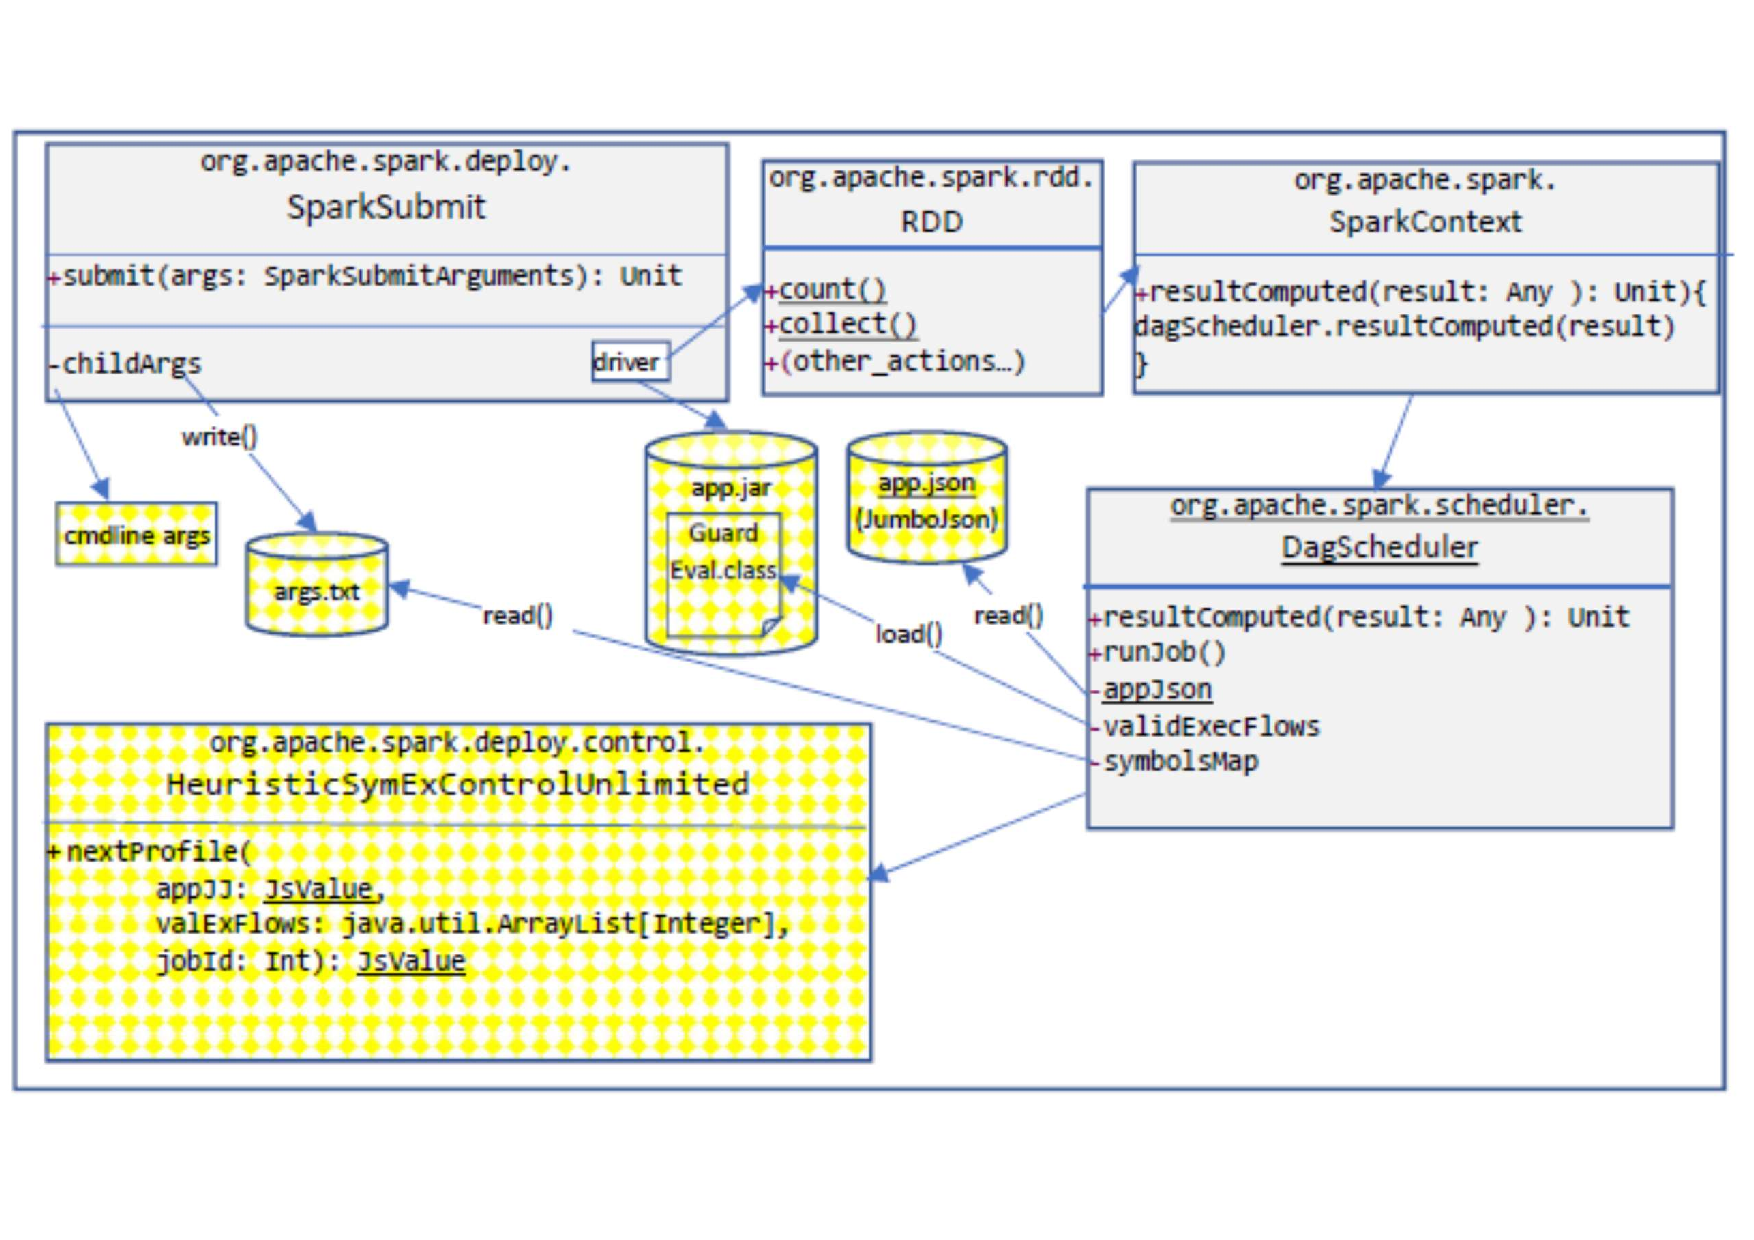
\includegraphics[width=12cm]{images/solution_impl_overview}
	\caption{Simplified solution components overview.}
	\label{fig:solution_impl_overview}
\end{figure}


\subsection{Backgound: Current xSpark Heuristic}\label{sec:impl_background}
%We recap here the information given in \MySec{sec:heuristic}.

xSpark uses a heuristic to compute per-stage deadlines and to estimate how many cores must be allocated for a stage to successfully fulfill the deadline. See \MySec{sec:heuristic} for an exhaustive description of its funcionality.
%At submission time three parameters: are collected: i) the application deadline, ii) the cluster size, and iii) the number of cores per worker node. Before executing the application, xSpark performs a feasibility check given the available resources. When a stage is submitted for execution, its deadline is computed \[deadline(sk) = \dfrac{\alpha\cdot ApplicationDeadline - SpentTime}{weight(sk)}\] where $SpentTime$ is the time already spent for execution and $\alpha$ a value between 0 and 1 that xSpark uses to be more conservative with respect to the provided ApplicationDeadline. The weight is computed 
%\[\begin{cases}
%w1(sk) = \#(RemainingStages + 1)\\
%w2(sk) = \dfrac{{\Sigma}_{{a}_{i=k}}^{k+{w}_{1}}duration(s_i)}{duration(sk)}\\
%weight(sk) = \beta\cdot w1(sk) + (1 - \beta) \cdot w2(sk)\\
%\end{cases}\]
%where w1 is the number of stages still to be scheduled (s included) and w2 is the rate between the duration of s and the duration of the remaining stages (s included). xSpark then proceeds to estimate how many cores are needed to execute the stage:
%\[estimatedCores(sk) = \lceil {\dfrac {inputRecords(sk)}{deadline(sk) \cdot nominalRate(sk)}}\rceil\]
%where inputRecords is the number of records that will be processed by sk and nominalRate is the number of records processed by a single core per second in stage sk.

%Since xSpark controls the resource allocation of a stage before and during the execution, the maximum amount of allocable cores needs to be greater than the estimated one, in order to be able to accelerate when progressing slower than expected 
%\[maxAllocableCores(sk) = overscale \cdot estimatedCores(sk)\]
%The final step determines the initial number of cores that should be assigned to the different executors. xSpark distributes the cores equally among the available workers by creating one executor per stage per worker. In this way, it is guaranteed that executor performances will be the same for each of them, and that xSpark can compute the same deadline for all the executors. The initial number of cores per executor is computed as
%\[initCorePerExec(sk) = \lceil\dfrac {maxAllocableCores(sk)}{overscale \cdot cq \cdot numExecutors}\rceil\cdot cq\]
%where $numExecutors$ is the number of executors and $cq$ is the $core\quantum$, a constant that defines the quantization applied to resource allocation, the smaller this value is, the more precise the allocation.

\subsection{Current xSpark Scheduling Limitation}\label{sec:impl_xspark_sched_limitation}
At runtime, an annotated DAG allows the xSpark scheduler function to comprehend how much work has already been completed and how much work still needs to be done. This means that xSpark can only optimize the allocation of the resources if the execution of all jobs of the application use the same DAG. This might not always be the case, for example when the code contains branches or loops, because these might need to be resolved in different ways at runtime. This is a severe limitation of the xSpark capability to manage real-world applications.

\section{Implementation Scope and Objective}\label{sec:impl_scope_objective}
The current work, by addressing the xSpark limitation explained above, aims at extending the scope of applicability of xSpark enhancing it with the capability to manage the case of applications that can potentially generate, at runtime, a different DAG at each execution. The code in this kind of applications includes conditional branches or iterative loops whose outcomes can only be resolved at runtime because they depend on user input values or results from previous computations that cannot be predicted or folded to constant values by the compiler. 
\subsection{Symbolic Execution}\label{sec:impl_symbolic_execution}
Executing a program symbolically means to simultaneously explore multiple paths that a program could take under different inputs. The key idea is to allow a program to take on symbolic – rather than concrete – input values. Execution is performed by a symbolic execution engine, which maintains for each explored control flow path: 
(i)	a first-order Boolean formula that describes the conditions satisfied by the branches taken along that path, and (ii) a symbolic memory store that maps variables to symbolic expressions or values. 

When a conditional branch is met, both sides of the branch are executed. Branch execution updates the formula, while assignments update the symbolic store. 
A symbolic execution tree is generated with an execution state associated with each node, containing the statement to be executed, the symbolic store, and the path conditions (a formula that expresses a set of assumptions on the symbols). The leaves of the tree identify the end of the computations, and tracing back from each leaf up to the root of the tree allows us to reconstruct, in reverse order, all the possible execution paths of the program. Our implementation exploits the funcionality provided by  \textit{GuardEvaluator}, an extension to Spark applications explained in \MySec{sec:guard_evaluator}, which is generated by an external implementation of the ligthweight symbolic execution algorithm  described in \MySec{sec:lightweight_symbolic_execution}.

\subsection{\tool vs. xSpark}
The first important difference between \tool and xSpark is in the profiling of the applications. xSpark requires the generation of a single DAG profile per application, while \tool requires a family of DAG profiles, one for each possible execution path, each of them associated to a unique set of “Path Conditions”. Profile information is collected in special JSON files, called "JSON profiles". \MyListing{lst:profile_example} shows an example of a JSON profile.
\lstinputlisting[
firstline=1,
lastline=141,
%float=thb,
language=python,
tabsize=2,
numbers=left,
numberstyle=\tiny,
stepnumber=1,
numbersep=5pt,
caption={Example of JSON profile.}, 
captionpos=t,
label=lst:profile_example
]{CodeFiles/CallsExample-1.json}

The profiling information for a \tool application is obtained by combining the JSON profiles, obtained by driving the application with different sets of input data so to drive the execution of all the possible execution paths, into a JSON file that we will call with a jargon “JumboJSON”, as shown in \MyFig{fig:jumboJSON_structure}.
\begin{figure}[tbhp]
	\hspace*{-2cm}
	\centering
	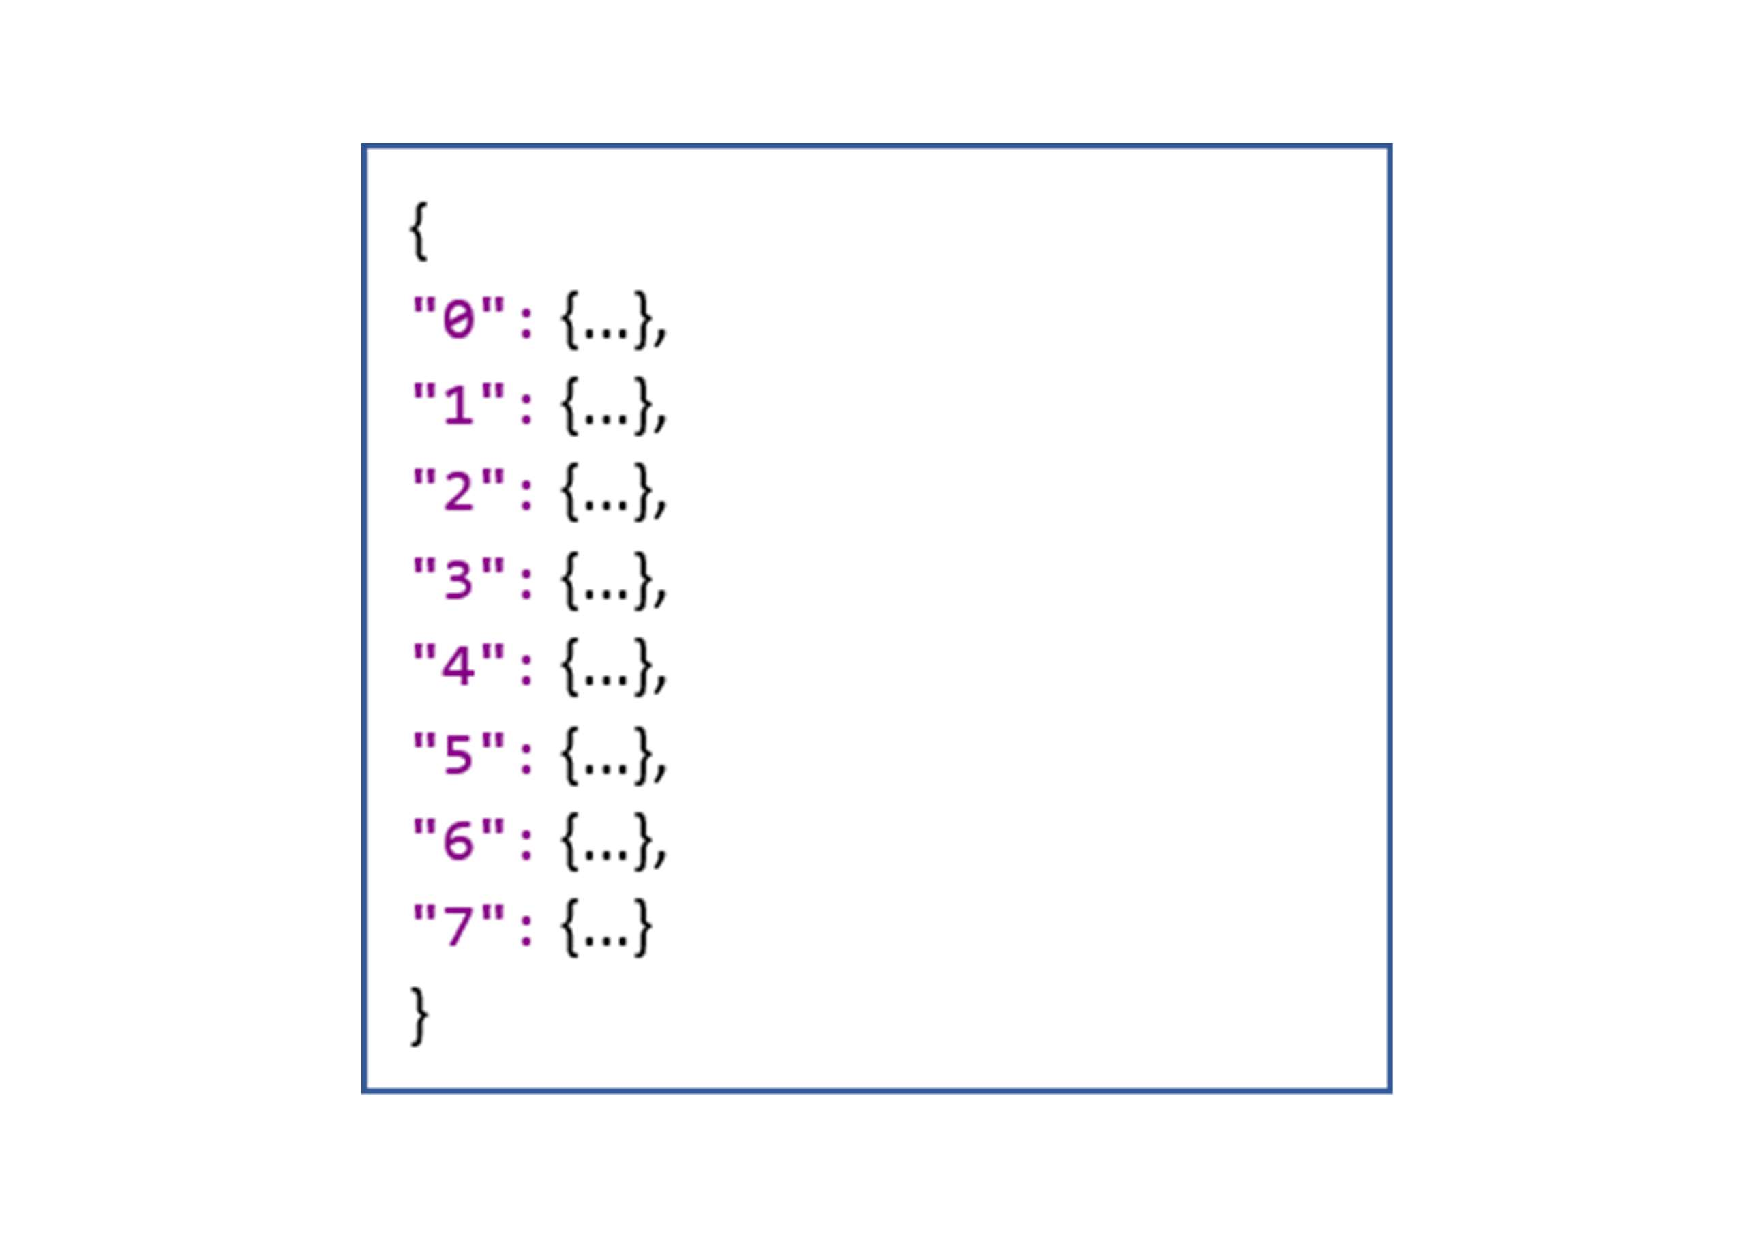
\includegraphics[width=18cm]{images/xsparksymb_profile_structure}
	\caption{Structure of profile JumboJSON. Each profile is identified by its profile id's {"$0$", "$1$", ...,"$7$"} and, in general, is characterized by its own number of stages and key values. Left and right images show the same JumboJSON profile where profile "$0$" (left) and profile "$1$" (right) are expanded, to show their difference in terms of number of stages ($6$ stages for profile $0$ and $3$ for profile $1$ ) and totalduration ($76,200$ ms for profile $0$ ms and  $43,000$ ms for profile $1$).}
	\label{fig:jumboJSON_structure}
\end{figure}
Futhermore, each single json profile is enhanced with information about the jobs composing the application, as shown in \MyFig{fig:profile_jobs_info}. 
\begin{figure}[tbhp]
	%\vspace*{-1cm}
	\hspace*{-1.7cm}
	\centering
	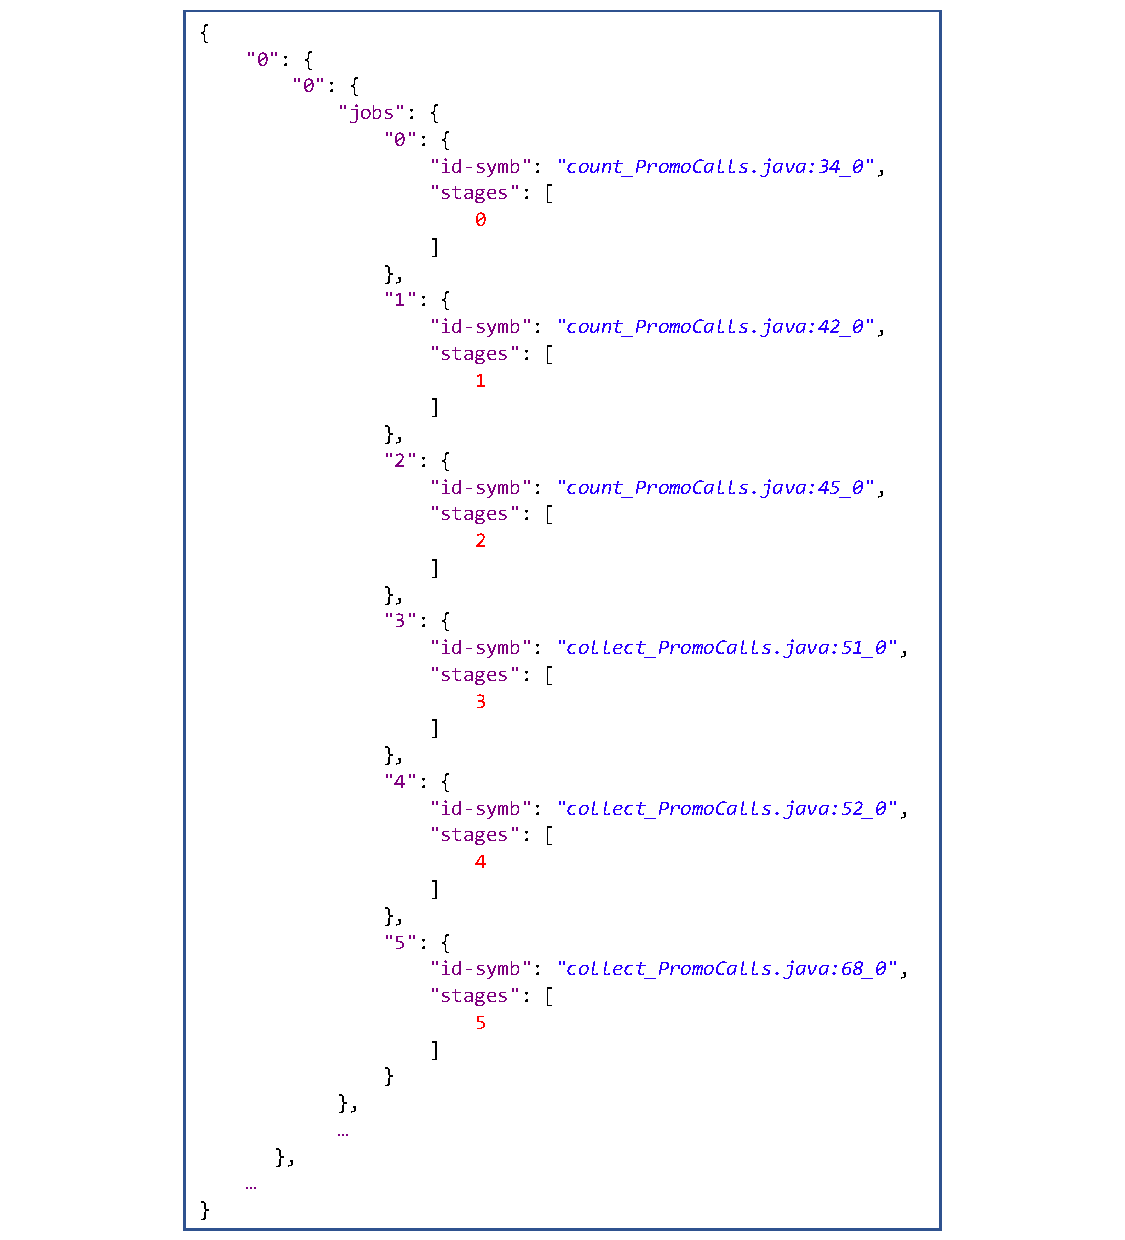
\includegraphics[width=15cm]{images/xsparksymb_profile_jobs_info}
	\caption{Information about jobs in json DAG profile.}
	\label{fig:profile_jobs_info}
\end{figure}
Inside \tool is kept a symbolic memory store that maps symbolic values (or symbols) to actual values. To this structure, initially empty, a new entry is added every time a symbolic value gets assigned a concrete value. Each entry is a key-value pair containing the symbol as key and the assigned value as value. The convention adopted for naming the symbols is the following:
\begin{itemize}
	\item \textbf{Commandline arguments}: prefix “arg\_” followed by an integer reflecting the position of the argument on the commandline. For example: “arg\_0”, “arg\_1” etc…
	\item \textbf{Program variables}: Spark action name followed by “\_”, followed by program name followed by “:”, followed by the program line number where the action is called, followed by “\_”, followed by an integer representing the number of times the action in the same line of code is being repeated. For example: "count\_PromoCalls.java:34\_2"
\end{itemize} 
\begin{table}[tbhp]
	\centering
	\caption{Example of Symbolic Memory Store contents.}
	\label{Table:impl_symbolic_memory_store_contents}
	\begin{tabular}{|c|c|c|}
		\hline
		\textbf{Entry\#} & \textbf{Key} & \textbf{Value} \\ \hline
		0	& arg\_0						&  100      \\ \hline
		1	& arg\_1						&  200      \\ \hline
		2	& arg\_2						&  300      \\ \hline
		3	& count\_PromoCalls.java:42\_0	& 2350      \\ \hline
		4	& count\_PromoCalls.java:45\_0	& 1920      \\ \hline
		5	& count\_PromoCalls.java:45\_1	& 3800      \\ \hline
	\end{tabular}
\end{table}
\MyTab{Table:impl_symbolic_memory_store_contents} shows an example of symbolic memory store contents during the execution of the application, run with three commandline arguments having value “100”, “200”, “300” and two spark actions already executed, of which the second was executed twice.
The application is also required to provide a class implementing a method called \texttt{evaluateGuards} that receives in input a Map of a symbolic memory store (as the one described above) and returns a list of the profile id’s whose DAG’s are still executable (i.e. they contain execution paths whose Path Conditions are satisfiable).

\subsection{A new Heuristic}\label{sec:new_heuristic}
\tool implements \texttt{HeuristicSymExControlUnlimited}, a 
new heuristic that extends \texttt{HeuristicControlUnlimited}. 
%\MyFig{fig:heuristic_simplified_class_diagram} below shows the simplified class diagram showing the relationships between the heuristic classes in the spark.deploy.control package.
The class diagram with the relationships between the heuristic classes is shown in \MyFig{fig:heuristic_class_diagram}. A new method, \texttt{nextProfile}, is implemented by the new heuristic. It takes the following input parameters:
\begin{enumerate}[$1) $] 
	\item a json containing the application profiles obtained by the concrete execution of every possible execution path of the application;
	\item a list of the profile id’s that are still satisfiable;
	\item the id of the job being submitted;
\end{enumerate}
and returns the json of the application profile to be used during the execution of the next job.
%\begin{figure}[tbhp]
%	\vspace*{-1cm}
%	\hspace*{-3cm}
%	\centering
%	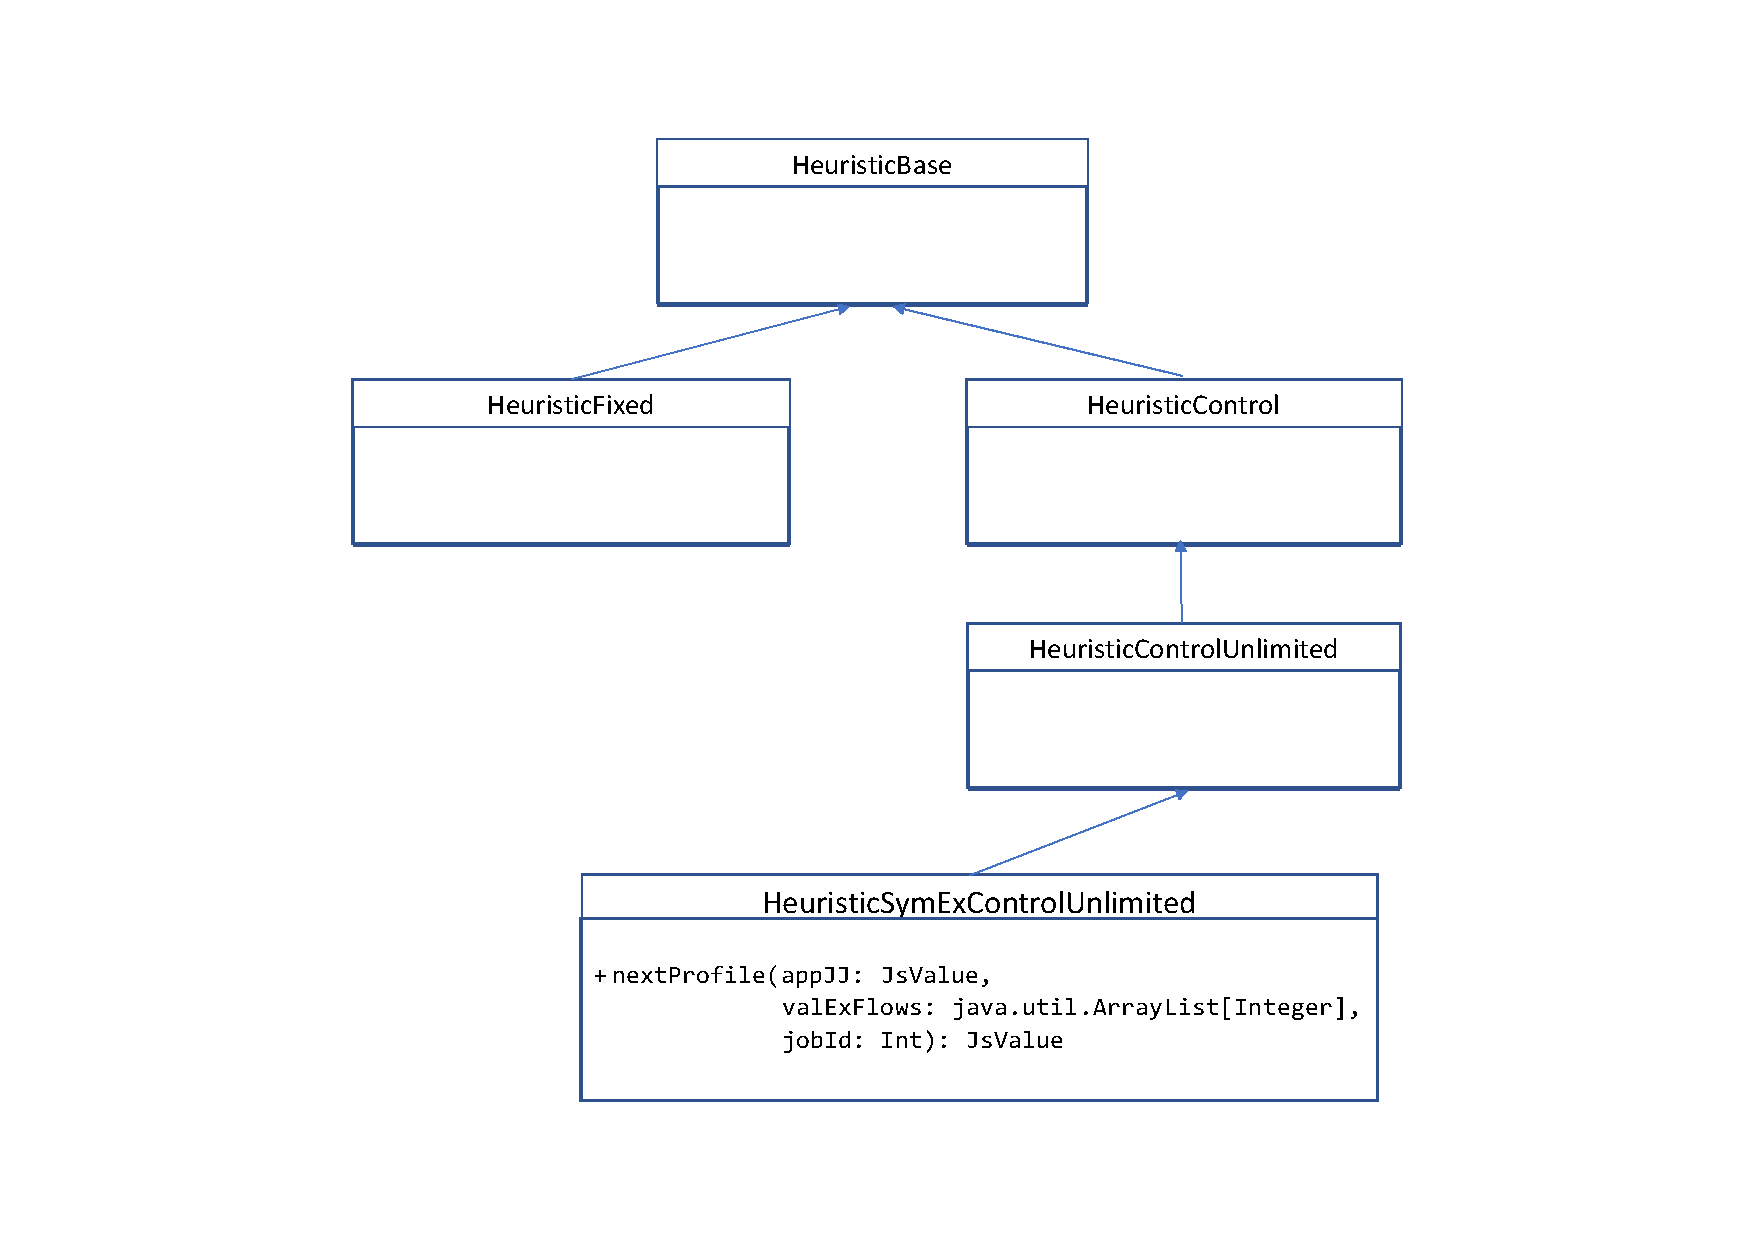
\includegraphics[width=16cm]{images/heuristic_simplified_class_diagram}
%	\vspace*{-1cm}
%	\caption{\tool Heuristic related simplified class diagram.}
%	\label{fig:heuristic_simplified_class_diagram}
%\end{figure}
Keeping in mind that the scheduler uses the \texttt{HeuristicSymExControlUnlimited} to estimate how many cores are needed to execute the stage, given the application deadline and the parameters in the application profile, we expect the new heuristic to choose the profile so as not to jeopardize the controller's ability to meet the deadline. This can be achieved by choosing a profile that will lead to not underestimate the cores needed to execute the remaining stages. All the following parameters seem to be good proxies for estimating the remaining computing effort:
\begin{verbatim}
1)	Number of remaining stages to be executed
2)	Sum of duration of remaining stages to be executed
3)	Weighted combination of 1 and 2 above
\end{verbatim}
The above parameters can be calculated using the data inside the application json profile. 
Current implementation of the heuristic uses proxy \#1 (number of remaining stages to be executed). It calculates the value for each of the satisfiable profiles, and then selects the profile associated to the maximum value of the proxy. This way, we supply the “worst case” profile to the heuristic, so that the stage deadline is not overestimated and consequently the number of cores to be assigned for the next stage execution is not underestimated.

\section{Application Parameters}\label{sec:application_parameters}
As explained in Chapter~\ref{chap:ProblemAndSolution}, the application parameters can be part of a path condition as they could have been associated to a symbol by the symbolic executor part of \dSymb. Hence, we have introduced in xSpark a mechanism to intercept and store these application parameters in the \tool \textit{Symbol Store}, as shown in \MyFig{fig:xsparkdagsymb}.  \MyListing{lst:SparkSubmit_submit} shows part of the code of method \textit{submit} of xSpark class \textit{SparkSubmit}, that was modified in order to read the values of the application's runtime arguments passed via the Spark \textit{submit} command and write them as separate lines to textfile \textit{args.txt}. This file is a component of the \textit{\model Store}. Records from this file are read by xSpark at a later stage, when lazily executing the application by means of job scheduling.
 
\lstinputlisting[
firstline=1,
lastline=13,
%float=thb,
language=scala,
tabsize=2,
numbers=left,
numberstyle=\tiny,
stepnumber=1,
numbersep=5pt,
caption={Changes to SparkSubmit method "submit".}, 
captionpos=t,
label=lst:SparkSubmit_submit
]{CodeFiles/SparkSubmit_submit.scala}

\section{Application Profiling}\label{sec:application_profiling}
As shown in \MyFig{fig:xsparkdagsymb}, for each set of input parameters identified by \dSymb a \textit{Launcher} is generated. A \textit{Launcher} is a Java class which contains the command to run the application with a specific set of arguments, which is in a 1:1 relationship with the application parameters of the corresponding \plan. An example of Launcher class is shown in \MyListing{lst:LauncherExample}. 

A \textit{Profiling} (see \MyFig{fig:xSparkExecFlow}
) of the application is done by running it with each \textit{Launcher}'s set of arguments. Each profiling run generates the corresponding \plan in a specialized JSON file. At the end of this process, all the generated \plans are packaged into another JSON file, in jargon called \textit{JumboJSON}, to form the \model. All the generated JSON files are then stored along with the \model \textit{Store} on the \textit{Spark Master} server. 
\lstinputlisting[
firstline=1,
lastline=42,
%float=thb,
language=java,
tabsize=2,
numbers=left,
numberstyle=\tiny,
stepnumber=1,
numbersep=5pt,
caption={Example of Launcher Code .}, 
captionpos=t,
label=lst:LauncherExample
]{CodeFiles/Launcher0.java}


\section{PEP*}\label{sec:getting_peps}
The previous version of xSpark required a single \plan to be present in the \textit{\plan Store}, so we had to modify the xSpark class \textit{DAGScheduler} to  account for the data in the \textit{JumboJSON file} that now contains all the \plans. To maintain backwards compatibility, a new variable was introduced, \texttt{JumboJson}, to hold the contents of the \model Store. The modified code is in charge of checking the \textit{heuristic type} in the \textit{SparkContext} instance \texttt{sc}, to understand if it should expect the contents of the \model Store to be a single \plan or a whole set of \plans representing a \model. The heuristic type is initialized with the value of the key \textit{spark.control.heuristic} specified in the xSpark configuration file \textit{spark-defaults.conf}. 

\lstinputlisting[
firstline=1,
lastline=10,
%float=thb,
language=scala,
tabsize=2,
numbers=left,
numberstyle=\tiny,
stepnumber=1,
numbersep=5pt,
caption={Changes to class DAGScheduler.scala - reading PEPs.}, 
captionpos=t,
label=lst:DAGScheduler-profile
]{CodeFiles/DAGScheduler_profile.scala}

\section{GuardEvaluator}\label{sec:guard_evaluator}
With the term \textit{GuardEvaluator} we collectively refer to the interface class \texttt{IGuardEvaluator} and its implementation class defining the \texttt{evaluateGuards} method, that is in charge of returning the list of valid profiles (\plans) when it is called with the HashMap of the known symbols and their values. The code of the  \texttt{IGuardEvaluator} interface is shown in \MyListing{lst:IGuardEvaluator}, while \MyListing{lst:GuardEvaluatorPromoCallsFile} shows an example of an implementation class and its method \texttt{evaluateGuards} for a specific application.
\lstinputlisting[
firstline=1,
lastline=9,
%float=thb,
language=java,
tabsize=2,
numbers=left,
numberstyle=\tiny,
stepnumber=1,
numbersep=5pt,
caption={Interface class IGuardEvaluator.}, 
captionpos=t,
label=lst:IGuardEvaluator
]{CodeFiles/IGuardEvaluator.java}
\lstinputlisting[
firstline=1,
lastline=142,
%float=thb,
language=java,
tabsize=2,
numbers=left,
numberstyle=\tiny,
stepnumber=1,
numbersep=5pt,
caption={Class GuardEvaluatorPromoCallsFile, implementing the IGuardEvaluator interface.}, 
captionpos=t,
label=lst:GuardEvaluatorPromoCallsFile
]{CodeFiles/GuardEvaluatorPromoCallsFile.java}


The application is in charge of providing the \textit{GuardEvaluator} as a java class, implementing the interface \texttt{IGuardEvaluator}, and packaged inside the jar of the application. This class is loaded dynamically at runtime by the new code added for this purpose to the xSpark class \texttt{DAGScheduler} and shown in \MyListing{lst:DAGScheduler_GuardEvaluator}.
\lstinputlisting[
firstline=1,
lastline=22,
%float=thb,
language=scala,
tabsize=2,
numbers=left,
numberstyle=\tiny,
stepnumber=1,
numbersep=5pt,
caption={Changes to class DAGScheduler.scala - Loading GuardEvaluator.}, 
captionpos=t,
label=lst:DAGScheduler_GuardEvaluator
]{CodeFiles/DAGScheduler_GuardEvaluator.scala}

\section{Symbol Store}\label{sec:symbol_store}
In order to take advantage of the symbolic execution, we need to maintain an updated   \textit{Symbol Store} containing all the symbols that can be part of a path condition and their associated determinations (assigned values). We added the code into the xSpark class \texttt{DAGScheduler} to abstractely represent the \textit{Symbol Store} as a  \textit{HashMap[String, Any]}. Each entry of this HashMap stores a \textit{known symbol} name and its value. By \textit{known symbol} we mean a symbol that has been associated to a value during the concrete execution of program code. Given this defintion, at the very beginning of the computation the only known symbols are the runtime arguments passed to the application. We added to the xSpark class \texttt{DAGScheduler} the code to read the arguments and their values and create the corresponding \textit{Symbol Store} entries. The code is shown in \MyListing{lst:DAGScheduler_symbol_store}, where we can notice that the first two arguments loaded when var \textit{iter} is set to negative values ($-2\ and -1$) are respectively the \textit{GuardEvaluator} class name and the application jar name, that are not symbols. They are not kept in the Symbol Store, instead they are used to initialize the variables \texttt{guardEvalClassname} and \texttt{appJar} which will be needed in a later step of the execution to identify the location and dynamically load the class implementing the \textit{GuardEvaluator} function.
\lstinputlisting[
firstline=1,
lastline=17,
%float=thb,
language=scala,
tabsize=2,
numbers=left,
numberstyle=\tiny,
stepnumber=1,
numbersep=5pt,
caption={Changes to class DAGScheduler.scala - Initializing Symbol Store.}, 
captionpos=t,
label=lst:DAGScheduler_symbol_store
]{CodeFiles/DAGScheduler_symbol_store.scala}
\section{Heuristic}\label{sec:impl_heuristic}
The heuristic used by xSpark is determined by the value of configuration parameter spark.control.heuristic and is an implementation of the class \texttt{HeuristicBase}, whose class diagram is shown in \MyFig{fig:heuristic_class_diagram}. In  \MyListing{lst:ControlEventListener_heuristic}, we can see that the heuristic \textit{HeuristicControl} is used by default, but other heuristics can be selected. \texttt{HeuristicFixed} and \texttt{HeuristicControlUnlimited} were already available in xSpark, while we implemented a new heuristic  \textbf{\texttt{HeuristicSymExControlUnlimited}} to exploit \textit{Symbolic Execution}.
\lstinputlisting[
firstline=1,
lastline=13,
%float=thb,
language=scala,
tabsize=2,
numbers=left,
numberstyle=\tiny,
stepnumber=1,
numbersep=5pt,
caption={Changes to class ControlEventListener.scala - selecting the heuristic.}, 
captionpos=t,
label=lst:ControlEventListener_heuristic
]{CodeFiles/ControlEventListener_heuristic.scala}
\begin{figure}[tbhp]
	\hspace*{-4cm}
	\centering
	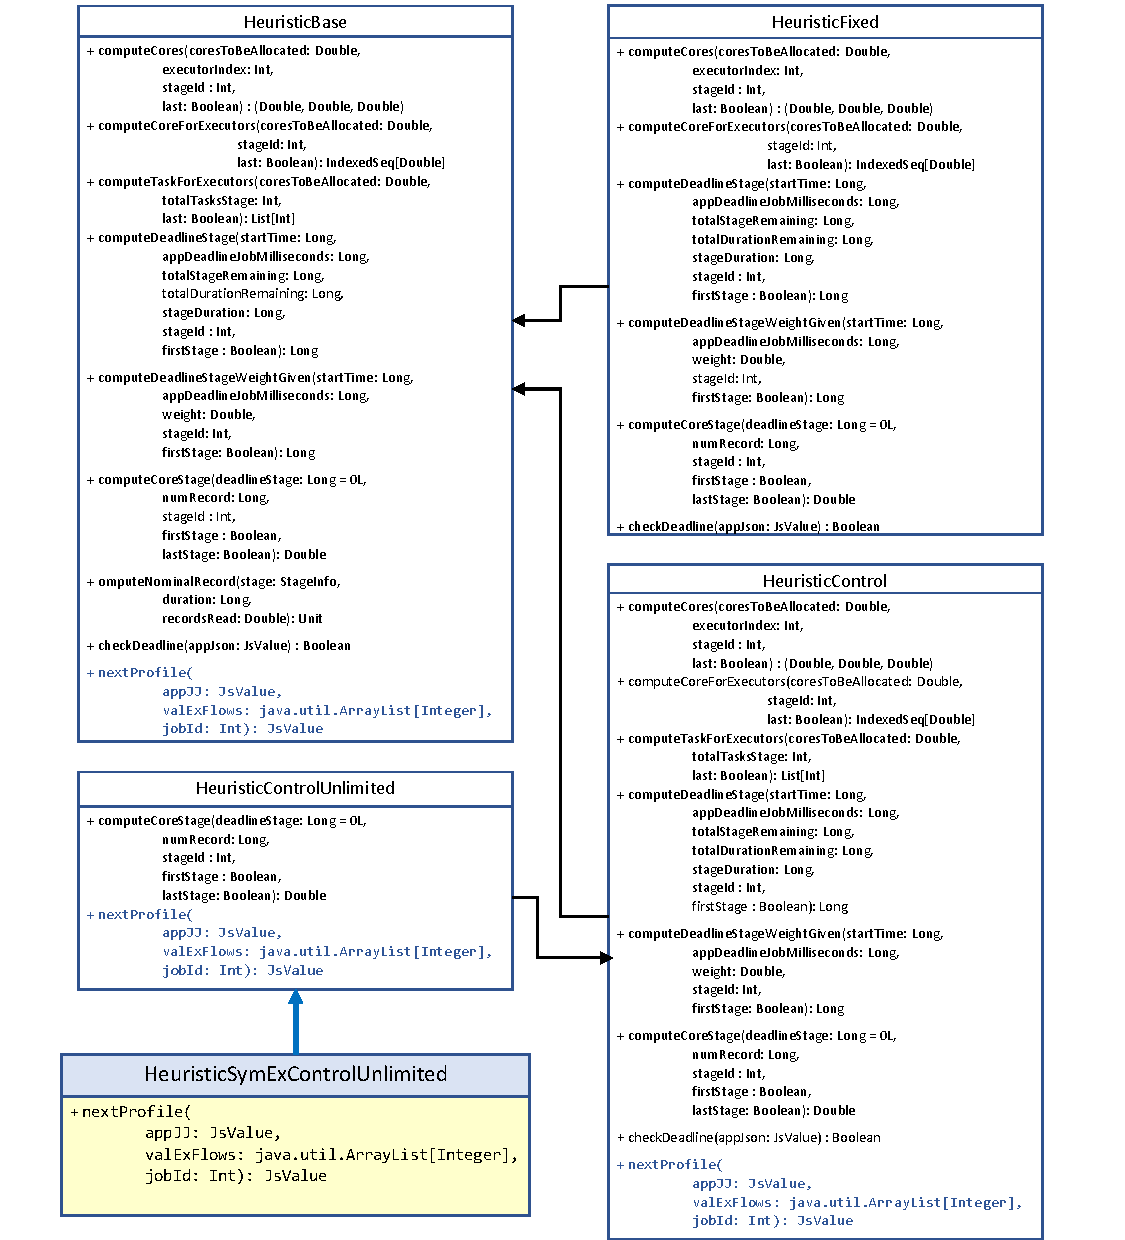
\includegraphics[width=20cm]{images/heuristic_class_diagram}
	\caption{Class diagram of Heuristic related classes.}
	\label{fig:heuristic_class_diagram}
\end{figure}
\texttt{HeuristicSymExControlUnlimited} extends \texttt{HeuristicControlUnlimited} by adding the implementation of a new method, \texttt{nextProfile}, taking parameters \texttt{appJson}, the \texttt{JumboJSON} containing the \model representation and \texttt{valExFlows}, a list containing the id's of the valid application profiles,(i.e. the list of the \plans whose path conditions still hold true), and returns the \plan of the profile to be used during the executing of the next scheduled job.
\lstinputlisting[
firstline=1,
lastline=27,
%float=thb,
language=scala,
tabsize=2,
numbers=left,
numberstyle=\tiny,
stepnumber=1,
numbersep=5pt,
caption={Class HeuristicSymExControlUnlimited.scala implementation.}, 
captionpos=t,
label=lst:HeuristicSymExControlUnlimited
]{CodeFiles/HeuristicSymExControlUnlimited.scala}
Class \texttt{HeuristicSymExControlUnlimited} implementation code is shown in \MyListing{lst:HeuristicSymExControlUnlimited}. The \plan selection is made by choosing the \textit{"worst case"} among the valid \plans, that is the \plan with the maximum number of stages still to be executed, as we want to be conservative and minimize the deadline violations. If we wanted to optimize another performance indicator, like minimum  resource utilization in absence of strict deadline commitment, we could choose the profile with an average number of remaining stages to be executed. 
  
\section{Symbols}\label{sec:guardevaluator}
As mentioned in \MySec{sec:symbol_store}, we have to update the Symbol Store everytime a variable associated to a symbol is evaluated by the concrete execution of the application. We adopted the convention to identify a symbol by the string \textit{arg\_n} if it refers to a runtime application argument, where n is the position of the argument (e.g. \textit{arg\_$0$}), or by a string obtained by concatenating its \textit{CallSite} and \textit{IterationNumber} separated by an underscore character \textit{"\_"}, where \textit{Call Site} is a string obtained by concatenating \textit{SparkActionName}, \textit{ApplicationClassName}, \textit{SourceLanguageName:SourceLineNumber} separated by an underscore character \textit{"\_"}, and  \textit{IterationNumber} is an integer starting from $0$ and incremented everytime a call is originated by the same \textit{CallSite}. i.e. the same line of code is re-executed (e.g. due to iterative loops). Examples of formal symbol names are shown in \MyFig{fig:symbol_name}.
\begin{figure}[tbhp]
	\centering
	\begin{lstlisting}[basicstyle=\ttfamily\scriptsize]
		          arg_0
		          count_PromoCalls_java:45_2
	\end{lstlisting}
	\caption{Example of symbol formal names.}
	\label{fig:symbol_name}
\end{figure}

As stated above, a symbol is identified by its \textit{CallSite}. This means that to identify the symbols we have to intercept calls coming from their  \textit{CallSite}. Since the values associated to a symbol can only be changed by xSpark \textit{actions} which delimit jobs, we added code to the method \texttt{runJob} of class \texttt{DAGScheduler} to extract the \textit{CallSite}, generate a symbol and push it in the \textit{Symbol Store} everytime the method \texttt{runJob} is called. The code is shown in \MyListing{lst:DAGScheduler_runJob}. 
\lstinputlisting[
firstline=1,
lastline=14,
%float=thb,
language=scala,
tabsize=2,
numbers=left,
numberstyle=\tiny,
stepnumber=1,
numbersep=5pt,
caption={Changes to class DAGScheduler.scala - method runJob.}, 
captionpos=t,
label=lst:DAGScheduler_runJob
]{CodeFiles/DAGScheduler_runJob.scala}
The variable \texttt{actionCallSite} is initialized using the value of the \texttt{callSite} parameter.
An auxilliary structure, the \textit{HashMap[String, Int]} \texttt{symbolMap} keeps track of every \texttt{actionCallSite} and counts how many times each of them has called the method runJob. The value of the count determines the suffix of each symbol. Symbols are initially assigned a \texttt{null} value, and stay in the symbol store waiting to be assigned the result of the \textit{action} originated from the \texttt{actionCallSite}. 

This task is performed by the new method \texttt{resultComputed}, that was added to the xSpark class \texttt{DAGScheduler}. \texttt{resultComputed} is called by the homonymous method, added to the class \texttt{SparkContext}, that passes to it the computed result of the action received from an \textit{action} method in the class \texttt{RDD}. 
%Since \textit{action}s are executed by specialized methods in the \texttt{RDD} xSpark class, 
Lastly, we have indeed modified the methods that execute the \textit{action}s in the \texttt{RDD} xSpark class by inserting a call to the method \texttt{resultComputed} of the \texttt{SparkContext} instance \texttt{sc} and passing to it the computed result of the action. 
%In turn, the method \texttt{resultComputed} in SparkContext calls \texttt{resultComputed} of class \texttt{DAGSCheduler}. 

Updating the value of \textit{symbols} in the \textit{Symbol Store} is not the only task fulfilled by the \texttt{resultComputed} method of class \texttt{DAGScheduler}. It also executes the method stored in the variable \texttt{guardEvalMethod} with the map of the known \textit{symbols} getting in return the variable \texttt{new\_validExecFlows} containing the list of valid profiles. It is also in charge of selecting the profile \texttt{appJson} to be used to run the next job. It fulfills this task by calling the method \texttt{nextProfile} of the \texttt{HeuristicSymExControlUnlimited} instance \texttt{heuristic} and passing to it the list of valid profiles. In returns, it gets the json profile to be used in the next job run, stored in the variable appJson. 

The new and modified methods are shown in Listings \ref{lst:DAGScheduler_resultComputed}, \ref{lst:SparkContext_resultComputed}, \ref{lst:RDD_actions}.

\lstinputlisting[
firstline=1,
lastline=21,
%float=thb,
language=scala,
tabsize=2,
numbers=left,
numberstyle=\tiny,
stepnumber=1,
numbersep=5pt,
caption={Changes to class DAGScheduler.scala - new  method resultComputed.}, 
captionpos=t,
label=lst:DAGScheduler_resultComputed
]{CodeFiles/DAGScheduler_resultComputed.scala}
\lstinputlisting[
firstline=1,
lastline=3,
%float=thb,
language=scala,
tabsize=2,
numbers=left,
numberstyle=\tiny,
stepnumber=1,
numbersep=5pt,
caption={Changes to class SparkContext.scala - new method resultComputed.}, 
captionpos=t,
label=lst:SparkContext_resultComputed
]{CodeFiles/SparkContext_resultComputed.scala}
\lstinputlisting[
firstline=1,
lastline=37,
%float=thb,
language=scala,
tabsize=2,
numbers=left,
numberstyle=\tiny,
stepnumber=1,
numbersep=5pt,
caption={Changes to class RDD.scala - modified methods count, collect and reduce.}, 
captionpos=t,
label=lst:RDD_actions
]{CodeFiles/RDD_actions.scala}

\section{Scheduling Jobs}\label{sec:scheduling_jobs}
Jobs in xSpark are delimited by \textit{actions} (e.g. \textit{count(), collect()  etc...)} and are composed by a number of stages, that reflect the \textit{transformations} operated on data. Data are abstracted as Resilient Distributed Datasets (\textit{RDD's} structures. As explained in Chapter~\ref{chap:Methodology}, the application parameters can be part of a path condition as they could have been associated to a symbol by the symbolic executor part of \dSymb. Hence, we have introduced in xSpark a mechanism to intercept and store these application parameters in the \tool \textit{Symbol Store}, as it was shown in \MyFig{fig:xsparkdagsymb}. The code listed in \MyListing{lst:SparkSubmit} was added to method \textit{submit} in xSpark module \textit{SparkSubmit} to read the values of the application's arguments passed via the Spark \textit{submit} command and write them as separate lines to textfile \textit{args.txt}. 

\section{Getting Results of Actions}\label{sec:getting_job_results}

\section{The Python Tool xSpark-dagsymb}\label{sec:xspark_dagsymb}

A tool exploiting symbolic execution techniques to safely run multi-dag
applications in xSpark. (https://github.com/gioenn/xSpark-dagsymb.git).
It combines two distinct functionalities, application profiling and
application execution, which are part of symbolic executor enabled
xSpark applications lifecycle, in one integrated tool called
\textbf{xSpark-dagsymb}.

The tool is composed by ten principal modules:
\textbf{xSpark\_dagsymb.py}, \textbf{launch.py}, \textbf{run.py},
\textbf{log.py}, \textbf{plot.py}, \textbf{metrics.py},
\textbf{configure.py}, \textbf{processing.py},
\textbf{average\_runs.py}, \textbf{process\_on\_server.py}, in addition
to the configuration files \textbf{credentials.json},
\textbf{setup.json}, \textbf{control.json}.

\hypertarget{core-functionality}{%
\subsection{Core Functionality}\label{core-functionality}}

The \textbf{launch.py} module manages the startup of spot request
instances on \emph{Amazon EC2} or virtual machines on \emph{Microsoft
Azure} and waits until the instances are created and are reachable from
the network via their public ip's. Subsequently the \textbf{run.py}
module receives as input the instances on which to configure the cluster
(\emph{HDFS} or \emph{Spark}), configures and runs the applications to
be executed and waits for the applications to complete. The module
\textbf{log.py} downloads and saves the logs created by the applications
run. The \textbf{plot.py} and \textbf{metrics.py} modules respectively
generate graphs and calculate metrics. The
\textbf{process\_on\_server.py} module can be called to remotely execute
the log analysis, graphs generation and metrics calculation on the
xSpark master server, and download the results to the client. This
option is very useful to speed-up the processing especially in case of
sizeable logfiles.

\hypertarget{cloud-environment-configuration}{%
\subsection{Cloud Environment
	Configuration}\label{cloud-environment-configuration}}

The Cloud environment must be properly initialized in order to allow
\textbf{xSpark\_dagsymb} to access and modify resources in the cloud.

\hypertarget{azure}{%
\subparagraph{Azure}\label{azure}}

Follow the instructions to create an identity called
\href{https://docs.microsoft.com/en-us/azure/azure-resource-manager/resource-group-create-service-principal-portal}{service
principal} and assign to it all the required permissions:

\begin{enumerate}
\def\labelenumi{\arabic{enumi})}
\item
Check that your account has the
\href{https://docs.microsoft.com/en-us/azure/azure-resource-manager/resource-group-create-service-principal-portal?view=azure-cli-latest\#required-permissions}{required
	permissions} to create an identity.
\item
Create an
\href{https://docs.microsoft.com/en-us/azure/azure-resource-manager/resource-group-create-service-principal-portal?view=azure-cli-latest\#create-an-azure-active-directory-application}{Azure
	Active Directory application}
\item
Get the
\href{https://docs.microsoft.com/en-us/azure/azure-resource-manager/resource-group-create-service-principal-portal?view=azure-cli-latest\#get-application-id-and-authentication-key}{\emph{Application
		ID} and an \emph{Authentication Key}}. The \emph{Application ID} and
\emph{Authentication Key} values replace respectively the
\emph{\textless{} AZ-APP-ID \textgreater{}} and the \emph{\textless{}
	AZ-SECRET \textgreater{}} values in the credentials.json file
described in the next paragraph.
\end{enumerate}

\hypertarget{tool-configuration}{%
\subsection{Tool Configuration}\label{tool-configuration}}

The \textbf{configure.py} module contains the Config class used to
instantiate configuration objects that are initialized with default
values. The \textbf{credentials.json} file contains \emph{Amazon EC2}
and/or \emph{Microsoft Azure} credential information. The
\textbf{setup.json} contains Cloud environment and \emph{Amazon EC2}
and/or \emph{Microsoft Azure} image parameters. The
\textbf{control.json} file contains xSpark controller configuration
parameters. Information in the \textbf{credentials.json},
\textbf{setup.json} and \textbf{control.json} files are used to
customize the configuration object used by other modules during the
application execution.

\begin{itemize}
\item
AWS and/or MS-Azure Credentials: Open the
\emph{credentials\_template.json} file and add the credentials for
\textbf{xSpark\_dagsymb} (see instructions below to retrieve missing
credentials):

\{ ``AzTenantId'': ``\textless{} AZ-TENANT-ID \textgreater{}'',
``AzSubscriptionId'': ``\textless{} AZ-SUBSCRIPTION-ID
\textgreater{}'', ``AzApplicationId'': ``\textless{} AZ-APP-ID
\textgreater{}'', ``AzSecret'': ``\textless{} AZ-SECRET
\textgreater{}'', ``AzPubKeyPath'': ``\textless{} AZ-PUB-KEY-PATH
\textgreater{}'', ``AzPrvKeyPath'': ``\textless{} AZ-PRV-KEY-PATH
\textgreater{}'', ``AwsAccessId'': ``\textless{} KEY-ID
\textgreater{}'', ``AwsSecretId'': ``\textless{} ACCESS-KEY
\textgreater{}'', ``KeyPairPath'': ``\textless{} KEY-PAIR-PATH
\textgreater{}'' \}
\end{itemize}

Save the file as \emph{credentials.json}.

\begin{itemize}
%\tightlist
\item
How to retrieve your Azure credentials (using the Azure Command Line
Interface):
\end{itemize}

Install the
\href{https://docs.microsoft.com/it-it/cli/azure/install-azure-cli?view=azure-cli-latest}{Azure
CLI}. Launch the following command from a console terminal:

\begin{verbatim}
$ az login
Note, we have launched a browser for you to login. For old experience with device code, use "az login --use-device-code"
\end{verbatim}

a browser authentication windows is open to allow you to login to the
Azure portal. If login is successful, you should get an output similar
to the following:

\begin{verbatim}
You have logged in. Now let us find all the subscriptions to which you have access...
[
{
"cloudName": "AzureCloud",
"id": "< AZ-SUBSCRIPTION-ID >",
"isDefault": true,
"name": "Microsoft Azure Sponsorship xx",
"state": "Enabled",
"tenantId": "< AZ-TENANT-ID >",
"user": {
"name": "*your_username*",
"type": "user"
}
}
]
\end{verbatim}

where you can pick the \emph{\textless{} AZ-SUBSCRIPTION-ID
\textgreater{}} and \emph{\textless{} AZ-TENANT-ID \textgreater{}}
parameters to be written in the \emph{credentials.json} file.

Launch the following command from a console terminal to create the
private and public RSA cryptography keys:

\begin{verbatim}
$ ssh-keygen -t rsa
\end{verbatim}

Save the generated files in your favorite folder and replace the values
\emph{\textless{} AZ-PUB-KEY-PATH \textgreater{}} and \emph{\textless{}
AZ-PRV-KEY-PATH \textgreater{}} in the \emph{credentials.json} file
respectively with the fully qualified file name of the public and the
private key.

\begin{itemize}
\item
Setup the xSpark and the Virtual Machine Cloud environment: Edit the
setup.json file to set the values to your need. The following is an
example using Microsoft Azure VM Cloud Service:

\{ ``Provider'': ``AZURE'', ``VM'': \{ ``Core'': 16, ``Memory'':
``100g'' \}, ``ProcessOnServer'': true, ``InstallPython3'': false,
``Aws'': \{ ``SecurityGroup'': ``spark-cluster'', ``Region'':
``us-west-2'', ``EbsOptimized'': true, ``Price'': ``0.015'',
``InstanceType'': ``m3.medium'', ``AwsRegions'': \{ ``eu-west-1'':
\{``ami'':``ami-bf61fbc8'', ``az'': ``eu-west-1c'', ``keypair'':
``simone'', ``price'': ``0.0035'' \}, ``us-west-2'': \{``ami'':
``ami-7f5ff81f'', ``snapid'': ``snap-4f38bf1c'', ``az'':
``us-west-2c'', ``keypair'': ``simone2'', ``price'': ``0.015''\} \}
\}, ``Azure'': \{ ``ResourceGroup'': ``xspark-davide-ap'',
``SecurityGroup'': ``cspark-securitygroup2'', ``StorageAccount'': \{
``Sku'': ``standard\_lrs'', ``Kind'': ``storage'', ``Name'':
``xsparkstoragedavide1'' \}, ``Subnet'': ``default'', ``NodeSize'':
``Standard\_D14\_v2\_Promo'', ``Network'': ``cspark-vnet2'',
``Location'': ``australiaeast'', ``NodeImage'': \{ ``BlobContainer'':
``vhd'', ``StorageAccount'': ``xsparkstoragedavide1'', ``Name'':
``vm2-os.vhd'' \} \}, ``Spark'': \{ ``ExternalShuffle'': ``true'',
``Home'': ``/opt/spark/'', ``LocalityWaitRack'': 0, ``CpuTask'': 1,
``LocalityWaitProcess'': 1, ``LocalityWait'': 0, ``LocalityWaitNode'':
0 \}, ``xSpark'': \{ ``Home'': ``/usr/local/spark/'' \}, ``SparkSeq'':
\{ ``Home'': ``/opt/spark-seq/'' \}
\item
Setup the Spark Controller parameters: Edit the control.json file to
set the values to your need. The following is an example:

\{\\
``Alpha'': 1.0, ``Beta'': 0.3, ``OverScale'': 2, ``K'': 50, ``Ti'':
12000, ``TSample'': 500, ``Heuristic'': ``CONTROL\_UNLIMITED'',
``CoreQuantum'': 0.05, ``CoreMin'': 0, ``CpuPeriod'': 100000 \}
\end{itemize}

\hypertarget{application-profiling}{%
\subsection{Application Profiling}\label{application-profiling}}

Profiling is the first logical phase of the performance testing
lifecycle. In profiling mode, Benchmarks are run using the ``vanilla''
Spark version. Then the \textbf{processing.py} module is called to
analyze the logs and create the ``application profile'', that is a JSON
file containing the annotated DAG of the executed stages plus additional
information intended to be used by the controller in the execution
phase. The \textbf{average\_runs.py} module is called to create a JSON
profile called *dagsymbmarkname\textgreater-app.json containing the
average values of the ``n'' profiles obtained by running the same
application ``n'' times. Finally, the file with the average profile is
uploaded to the xSpark configuration directory on the master server.

\hypertarget{application-execution}{%
\subsection{Application Execution}\label{application-execution}}

Benchmarks are executed using
\href{https://github.com/gioenn/xSpark.git}{xSpark}, and require the
application profile \emph{dagsymbmarkname}-app.json to be present in the
xSpark configuration directory. The name of the application and the
parameters to modify its default configuration can either be specified
as commandline arguments to the \emph{submit} command, or can be
inserted into JSON format ``experiment files'' and passed as commandline
arguments to the \emph{launch\_exp} command. As an example, an
experiment files for Pagerank , one for KMeans and one for
AggregateByKey are shown here below:

PageRank experiment file example:

\begin{verbatim}
{
"Deadline": 148080,
"BenchmarkName": "PageRank",
"BenchmarkConf": {
"NumOfPartitions": 1000,
"NumV": 35000000,
"Mu": 3.0,
"Sigma": 0.0,
"MaxIterations": 1,
"NumTrials": 1     
}
}
\end{verbatim}

KMeans experiment file example:

\begin{verbatim}
{
"Deadline": 116369,
"BenchmarkName": "KMeans",
"BenchmarkConf": {
"NumOfPartitions": 1000,
"NumOfPoints": 100000000,
"NumOfClusters": 10,
"Dimensions": 20,
"Scaling": 0.6,
"MaxIterations": 1
}
}
\end{verbatim}

AggregateByKey experiment file example:

\begin{verbatim}
{
"Deadline": 124000,
"BenchmarkName": "scala-agg-by-key",
"BenchmarkConf": {
"ScaleFactor": 5
}
}
\end{verbatim}

\hypertarget{download-requirements}{%
\subsection{Download \& Requirements}\label{download-requirements}}

\begin{verbatim}
$ git clone https://github.com/gioenn/xSpark-dagsymb.git
$ cd xSpark-dagsymb
$ pip3 install -r requirements.txt"
\end{verbatim}

\hypertarget{xspark-dagsymb-commands}{%
\subsection{xSpark-dagsymb commands}\label{xspark-dagsymb-commands}}

\href{https://github.com/gioenn/xSpark-dagsymb}{xSpark-dagsymb} run
command syntax:

\begin{verbatim}
$ cd xSpark-dagsymb
$ python3 xSpark_dagsymb.py *command [*args*]*
\end{verbatim}

\hypertarget{command-args-syntax}{%
\subparagraph{*command {[}*args*{]}*
	syntax:}\label{command-args-syntax}}

\begin{verbatim}
[setup | reboot | terminate | log | profiling | time_analysis | check | 
profile | submit | launch_exp] [*args*]
\end{verbatim}

where *args* is a set of command-specific arguments list or options.

\hypertarget{setup-command-syntax}{%
\subparagraph{\texorpdfstring{\emph{setup} command
		syntax:}{setup command syntax:}}\label{setup-command-syntax}}

\begin{verbatim}
setup [hdfs | spark | all | generic] {[-n | --num-instances] *numinstances*} 
{[-y |  --assume-yes]}
\end{verbatim}

where *numinstances* is the number of nodes to add to the specified
cluster (default is 5), \emph{-y} or \emph{--assume-yes} option sets
default affirmative answer to interactive confirmation requests.

\hypertarget{reboot-command-syntax}{%
\subparagraph{\texorpdfstring{\emph{reboot} command
		syntax:}{reboot command syntax:}}\label{reboot-command-syntax}}

\begin{verbatim}
reboot [hdfs | spark | all | generic]
\end{verbatim}

reboots all nodes in the specified cluster.

\hypertarget{terminate-command-syntax}{%
\subparagraph{\texorpdfstring{\emph{terminate} command
		syntax:}{terminate command syntax:}}\label{terminate-command-syntax}}

\begin{verbatim}
terminate [hdfs | spark | all | generic]
\end{verbatim}

deletes (destroyes) all nodes and their connected resources in the
specified cluster.

\hypertarget{check-command-syntax}{%
\subparagraph{\texorpdfstring{\emph{check} command
		syntax:}{check command syntax:}}\label{check-command-syntax}}

\begin{verbatim}
check [hdfs | spark | all | generic]
\end{verbatim}

checks the status of all nodes in the specified cluster.

\hypertarget{profile-command-syntax}{%
\subparagraph{\texorpdfstring{\emph{profile} command
		syntax:}{profile command syntax:}}\label{profile-command-syntax}}

\begin{verbatim}
profile [*exp_file_paths*] {[-r | --num-runs] *numruns*} {[-R | --reuse-dataset]} 
{[-q | --spark-seq]}      
\end{verbatim}

where *exp\_file\_paths* is a non-empty space separated list of
experiment file paths, *numruns* is the number of times to repeat the
profiling for each experiment file (default is 1), \emph{-R} or
\emph{--reuse-dataset} option instructs xSpark to reuse (not to delete)
application data in hdfs master node, \emph{-q} or \emph{--spark-seq}
option instructs xSpark to use Spark data sequencing home directory.

\hypertarget{submit-command-syntax}{%
\subparagraph{\texorpdfstring{\emph{submit} command
		syntax:}{submit command syntax:}}\label{submit-command-syntax}}

\begin{verbatim}
submit [*exp_file_paths*] {[-r | --num-runs] *numruns*} {[-R | --reuse-dataset]}       
\end{verbatim}

where *exp\_file\_paths* is a non-empty space separated list of
experiment file paths, *numruns* is an integer specifying the number of
times to repeat the profiling for each experiment file (default is 1),
\emph{-R} or \emph{--reuse-dataset} option instructs xSpark to reuse
(not to delete) application data in hdfs master node.

\hypertarget{launch_exp-command-syntax}{%
\subparagraph{\texorpdfstring{\emph{launch\_exp} command
		syntax:}{launch\_exp command syntax:}}\label{launch_exp-command-syntax}}

\begin{verbatim}
launch_exp {[-e | --executors] *numexecutors*} {[-b | --application] [pagerank | kmeans | 
sort_by_key]} {[-v | --variable-parameter] *bpar*} 
{[-n | --num-instances] *numinstances*} 
\end{verbatim}

where *numexecutors* is an integer specifying the maximum number of
executors to be used in the experiments, *bpar* is a variable parameter
representing num\_v for pagerank, num\_of\_points for kmeans,
scale\_factor for sort\_by\_key, \emph{-r} or \emph{--num-runs} is the
number of times the specified application is run, \emph{-p} or
\emph{--num-partitions} is the number of partitions for each task,
\emph{-P} or \emph{--profile} instructs xSpark to perform the profiling
at the end of the experiments, \emph{-R} or \emph{--reuse-dataset}
option instructs xSpark to reuse (do not delete) application data in
hdfs master node.

\hypertarget{log_profiling-command-syntax}{%
\subparagraph{\texorpdfstring{\emph{log\_profiling} command
		syntax:}{log\_profiling command syntax:}}\label{log_profiling-command-syntax}}

\begin{verbatim}
log_profiling {[-L | --local]}
\end{verbatim}

where \emph{-L} or \emph{--local} option instructs xSpark use default
local output folders.

\hypertarget{time_analysis-command-syntax}{%
\subparagraph{\texorpdfstring{\emph{time\_analysis} command
		syntax:}{time\_analysis command syntax:}}\label{time_analysis-command-syntax}}

\begin{verbatim}
time_analysis {[-i | --input-dir] *dir*}
\end{verbatim}

where \emph{dir} is the directory where the log files are located.

\hypertarget{example-profile-and-test-pagerank}{%
\subsection{Example: Profile and Test
	PageRank}\label{example-profile-and-test-pagerank}}

\begin{enumerate}
\def\labelenumi{\arabic{enumi})}
\item
Create the credential.json file as instructed above.
\item
Configure the setup.json file as instructed above.
\item
Configure the control.json file as instructed above.
\item
Create and initialize a hdfs cluster with 5 nodes:

\$ python3 xSpark\_dagsymb.py setup hdfs -n 5
\item
Create and initialize a spark cluster with 5 nodes:

\$ python3 xSpark\_dagsymb.py setup spark -n 5
\item
Create \emph{experiment.json} file with the the following contents:

\{ ``Deadline'': 148080, ``BenchmarkName'': ``PageRank'',
``BenchmarkConf'': \{ ``NumOfPartitions'': 1000, ``NumV'': 35000000,
``Mu'': 3.0, ``Sigma'': 0.0, ``MaxIterations'': 1, ``NumTrials'': 1\\
\} \}
\item
Run the Profiling with 6 iterations:

\$ python3 xSpark\_dagsymb.py profile experiment.json -r 6 -R
\item
Run the Application Test with 5 iterations:

\$ python3 xSpark\_dagsymb.py submit experiment.json -r 5 -R
\end{enumerate}

\hypertarget{todo}{%
\subsection{TODO}\label{todo}}

\begin{itemize}
%\tightlist
\item[$\square$]
complete this file with installation instructions for AWS
\item[$\square$]
clean-up code
\end{itemize}
